\subsection{Постановка задачи}
1.5. Реализовать алгоритм QR – разложения матриц в виде программы. На его основе разработать программу, реализующую QR – алгоритм решения полной проблемы собственных значений произвольных матриц, задавая в качестве входных данных матрицу и точность вычислений. С использованием разработанного программного обеспечения найти собственные значения матрицы.

{\bfseries Вариант:} 19
\begin{equation}
      \begin{pmatrix}
        0 & -1 & 3\\
        -1 & 6 & -3\\
        -8 & 4 & 2
      \end{pmatrix}
\end{equation}
\pagebreak

\subsection{Результаты работы}

\begin{figure}[h!]
\centering
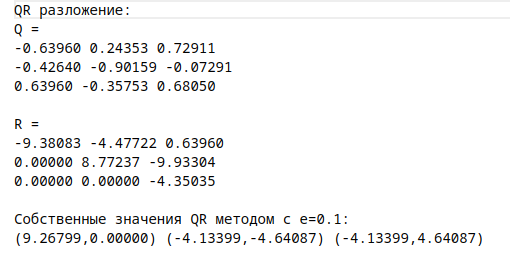
\includegraphics[width=.5\textwidth]{lab1.5}
\caption{Вывод в консоли}
\end{figure}
\pagebreak

\vfill

\subsection{Исходный код}

\lstinputlisting[title=\texttt{Lab1.5.cpp}]{../stud/saifullin/task1.5/Lab1.5.cpp}
\pagebreak
